\section{Introduction} % 

In the past decade, Artificial Neural Networks (ANNs) have become increasingly
popular, with advances in the area affecting almost every sector of computing.
Deep Neural Networks (DNNs) \--- deeper, more complex models than their
`shallow' counterparts \--- have progressed from being academic curiosities to
being the cornerstone of many modern technologies~\cite{deep_learning_overview},
with work showing that deeper networks tend to give better results than wide
networks~\cite{VGG}. Given this newfound relevance, many researchers have
devoted a lot of time optimizing these algorithms, constantly trying to improve
them for different accelerator technologies and platforms. Even long before
accelerators, many efforts in trying to parallelize neural networks were
made~\cite{10.1007/BFb0024235}.  While the new resurgence of machine learning
(ML) partially came from the generalized availability of hardware accelerators
like GPUs, there are still many innovations being made for CPUs. An example of
this is Facebook's new Speech-to-Text (stt) system that runs on
CPUs~\cite{fbcpu} and is aimed at home assistants that cannot rely on large and
power-hungry accelerators.  As ML algorithms are getting larger, there are also
continued efforts to apply machine learning techniques to simpler hardware.
Thus, for the foreseeable future, optimizing ML algorithms on various platforms
will remain an active area of research.

In this section we will discuss the various algorithms used in machine learning.
In Section~\ref{sec:ann} we will discuss Artificial Neural Networks and the
underlying theory behind them. In Section~\ref{sec:method} we will discuss how
we implemented our network and our design choices. In Section~\ref{sec:results}
we will discuss the results and the optimizations we achieved from our
parallelization efforts. Finally, in Section~\ref{sec:conclusions} we conclude
the work and summarize our findings.

\subsection{Artificial Neural Networks}\label{sec:ann}

This section presents the theory behind ANNs and the Gradient Descent (GD)
algorithm that is commonly used to train them.

\subsubsection{Perceptrons}

The Perceptron, also referred to as ``neuron'', is the basic unit of an ANN. It
is a mathematical function that was inspired by the biological neurons in the
human brain~\cite{rosenblatt1958perceptron}. Its mathematical formula is presented in Equation~\ref{eq:perceptron}. It consists of a dot product between a feature vector $x$
and a weights vector $w$. The resulting dot product of these vectors is then fed
into a function $g$ known as \textit{activation}~\cite{activation_functions} which yields the output
$\hat{y}$ of the neuron.

\begin{align}
    \hat{y} = g\left(\sum^n_{i=0} w_ix_i\right)
    \label{eq:perceptron}
\end{align}

Perceptrons can be used to solve regression (estimating real values) or
classification problems (discrete number of classes). The feature vectors are
obtained directly from the function being estimated or the dataset being
classified. The weights vector can be initialized to a vector of zeros, however,
it is common to initialize it using random numbers in the range $[0,1)$ drawn
from a uniform distribution. By providing random initializations networks
typically converge faster and generalize better.

As for the activation function, Figure~\ref{fig:activations} presents a few
examples of commonly used ones~\cite{activation_functions}. The bottom-right image in
Figure~\ref{fig:activations} shows an example of a linear activation in the form
of the Identity function. The other three examples represent non-linear
activations: the Sigmoid (bottom-left) function yields an output between 0 and
1; the Hyperbolic Tangent function (up-left) has an output between -1 and 1; and
the Rectified Linear Unit, or ReLU, (up-right) is a modified Identity that
changes negative values to 0.

\begin{figure}[!htbp]
    \centering
    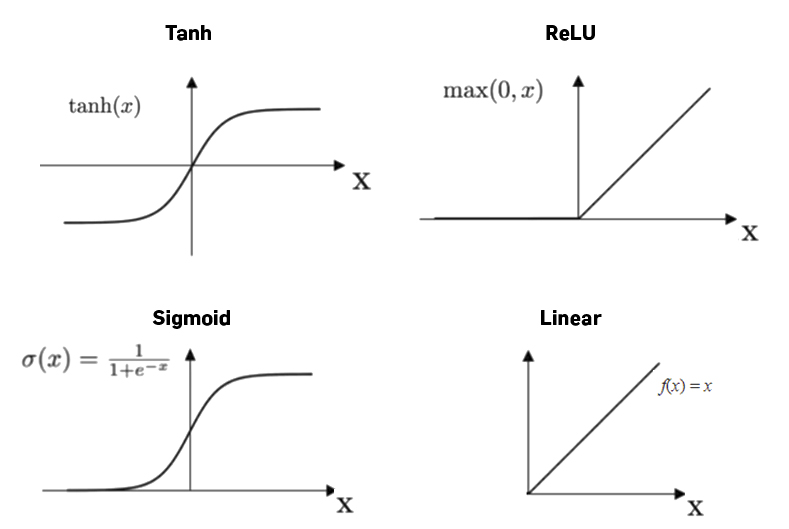
\includegraphics[width=.5\textwidth]{Images/activations.jpg}
    \caption{Examples of activation functions.}
    \label{fig:activations}
\end{figure}

The activation function plays a crucial role because it actually determines the
sort of problems that a perceptron is able to solve. If a linear (Identity,
Step, Sign) activation function is used, a single perceptron is only able to
solve ``linearly separable'' problems, that is, problems in which the classes
can be successfully separated by a hyper-plane (Figure
\ref{fig:linear_vs_non_linear} left). On the other hand, by using a non-linear
(Sigmoid, Tanh, ReLU) activation a more flexible decision boundary is created
and, thus, more complex problems can be solved (Figure
\ref{fig:linear_vs_non_linear} right).

\begin{figure}[!htbp]
    \centering
    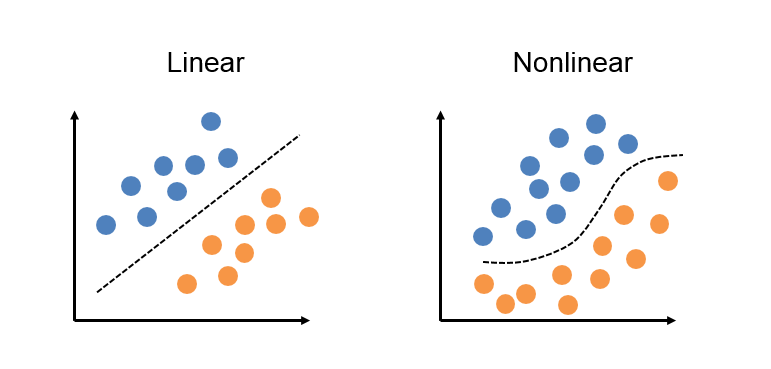
\includegraphics[width=.5\textwidth]{Images/linear_vs_non_linear.png}
    \caption{Linearly-separable vs non-linearly separable.}
    \label{fig:linear_vs_non_linear}
\end{figure}

\subsubsection{Training Perceptrons with Gradient Descent}
 
It is safe to assume that the initial output of the perceptron $\hat{y}$,
obtained with the initial state of the weights vector, will be different than
the expected output $y$ (label). So, in order to improve these predictions, the
perceptron needs to be ``trained''. Training a perceptron basically means
iteratively modifying the weights vector so that the outputs start to
approximate the expected ones. This training process is illustrated in
Figure~\ref{fig:perceptron_train}: using the the expected output $y$ and the
obtained output $\hat{y}$ an error measure is computed and used to modify the
weights. This process is repeated until the outputs fulfill a  given convergence
criteria or a maximum number of iterations is reached.
 
\begin{figure}[!htbp]
    \centering
    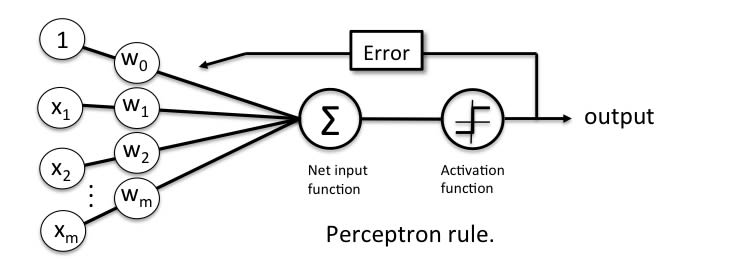
\includegraphics[width=.5\textwidth]{Images/perceptron_learning.jpg}
    \caption{Perceptron training.}
    \label{fig:perceptron_train}
\end{figure}

The Gradient Descent (GD) algorithm~\cite{gradient_descent} is an optimization technique that is used to
train perceptrons. The main idea behind GD is to update the weights in the
direction of the gradient of the function used to compute the error between the
perceptron's outputs and the expected ones. This function is commonly referred
to as \textit{Loss} function~\cite{loss_functions}. The actual problem being solved determines the
type of loss function that should be used. For example, in regression problems
the Mean Squared Error (MSE) loss function is a typical choice. For binary
classification problems, Binary Cross-Entropy loss or Hinge loss are good
options. In multi-class classification problems, Cross-Entropy loss is the
default alternative.

The general formula for the GD method is shown in Equation~\ref{eq:gd_formula}. First, the derivative of the chosen loss function $L$ with respect to the weights vector $w$ is obtained. Then it is multiplied by a scalar parameter $\gamma$ known as \textit{learning rate}. Finally, the weights are updated using this product.

\begin{align}
    w = w - \gamma \frac{d}{d_w}L
    \label{eq:gd_formula}
\end{align}

While the formula for GD is straightforward, obtaining the derivative of the
loss function with respect to the weights is not always trivial as the chain
rule of derivatives is needed. For example, Equation~\ref{eq:bce_loss} shows the
mathematical formula of the Binary Cross-Entropy loss function.

\begin{align}
    L(w) = y * \log(\hat{y}) + (1 - y) * \log(1 - \hat{y})
    \label{eq:bce_loss}
\end{align}

If we assume a perceptron using the sigmoid activation function, the derivative
of the loss is obtained in the following manner:

\begin{align}
    d &= w^T x \\
    \hat{y} &= \sigma(d) = \frac{1}{1 + e^{-d}} \\
    \frac{\partial L(w)}{\partial w} &= \frac{\partial L(w)}{\partial \hat{y}} \cdot \frac{\partial \hat{y}}{\partial d} \cdot \frac{\partial d}{\partial w}\\
    \frac{\partial L(w)}{\partial \hat{y}} &= -\left(\frac{y}{\hat{y}} - \frac{1
    - y}{1 - \hat{y}}\right) = \frac{\hat{y} - y}{\hat{y}(1-\hat{y})} \\
    \frac{\partial \hat{y}}{\partial d} &= \hat{y}(1 - \hat{y}) \\
    \frac{\partial d}{\partial w} &= x \\
    \frac{\partial L(w)}{\partial w} &= x^T(\hat{y}-y)
\end{align}

There are some variations to the GD algorithm, each with its own strengths and
weaknesses. In Stochastic Gradient Descent (SGD)~\cite{gradient_descent}, the weights are updated for
each training sample in the dataset, i.e. the output of one feature vector is
obtained, the derivative of the loss function for that output is computed, and
the weights are updated according to the GD formula. This version is, of course,
suitable for online training or when the training dataset is so big that it
cannot fit in memory all at once. However, the constant weight updates produce a
the chaotic behaviour shown in Figure~\ref{fig:sgd} as each training sample
attempts to pull in its own direction.

\begin{figure}[!htbp]
    \centering
    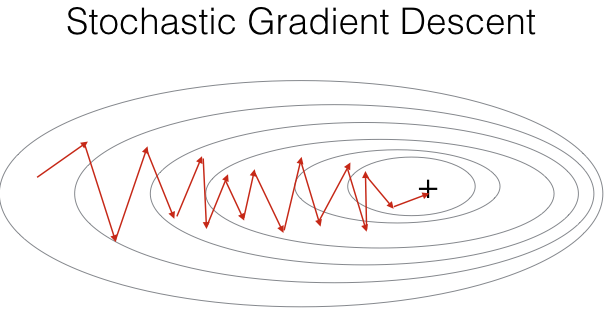
\includegraphics[width=.4\textwidth]{sgd.png}
    \caption{SGD convergence behaviour.}
    \label{fig:sgd}
\end{figure}

The (Mini) Batch Gradient Descent (BGD)~\cite{gradient_descent} variation instead splits the training
samples into small-sized batches and only updates the weights once per each
batch. Thus, using BGD makes the algorithm behave more smoothly with less
pronounced changes in its path towards convergence as it is shown in
Figure~\ref{fig:bgd}.

\begin{figure}[!htbp]
    \centering
    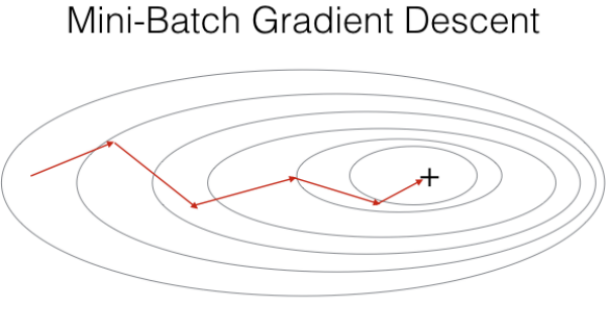
\includegraphics[width=.4\textwidth]{bgd.png}
    \caption{BGD convergence behaviour.}
    \label{fig:bgd}
\end{figure}

\subsubsection{Multi-layer Perceptrons}

There are, of course, limitations to what a single perceptron can accomplish no
matter the activation function used. Figure~\ref{fig:unsolvable} presents one of
such cases in which a classification problem cannot be solved by a single
perceptron, which is because multilayer perceptron networks are universial
approximators~\cite{HORNIK1989359}. The dataset shown
in the figure contains points in two dimensions labeled as two distinct classes
identified by the colors blue and orange. As can be observed, the blue class is
``contained'' within the orange class and, as such, it is impossible for a
single perceptron to define a decision boundary, even a non-linear one, that
will correctly classify all of the points. 

\begin{figure}[!htbp]
    \centering
    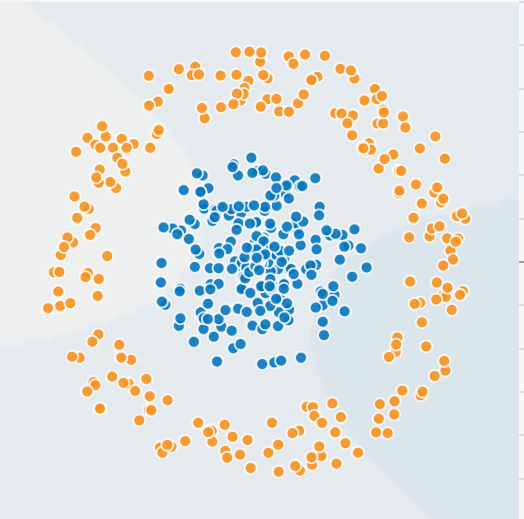
\includegraphics[width=.35\textwidth]{Images/circles.png}
    \caption{Class contained within the other.}
    \label{fig:unsolvable}
\end{figure}

Figure~\ref{fig:one_perceptron} presents the decision boundary created by a
single perceptron using a sigmoid activation. In the figure, it can be observed
that the resulting decision boundary correctly classifies most of the blue-class
points. However, it incorrectly classifies the vast majority of the orange-class
points.

\begin{figure}[!htbp]
    \centering
    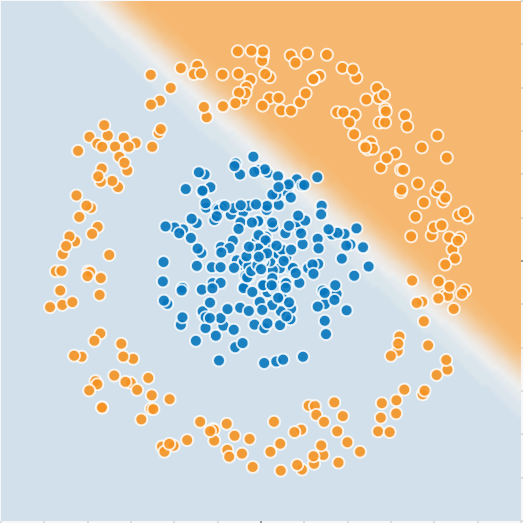
\includegraphics[width=.35\textwidth]{Images/circles_perceptron.png}
    \caption{One perceptron solution.}
    \label{fig:one_perceptron}
\end{figure}

In problems such as the this one using an ANN, also known as Multi-Layer
Perceptrons (MLPs), becomes necessary. A MLP consists in several perceptrons
connected together to form a ``network''. In the literature, there exist
multiple ways in which the perceptrons can be arranged to form different
architectures~\cite{deep_learning_overview}. However, in this work we focus on
the architecture known as ``Feed-Forward Neural Network'' (FFNN)~\cite{ffnn},
shown in Figure~\ref{fig:ffnn}. In FFNNs, all neurons in one layer are connected
to all of the neurons in the following layer, hence the name Feed-Forward.

\begin{figure}[!htbp]
    \centering
    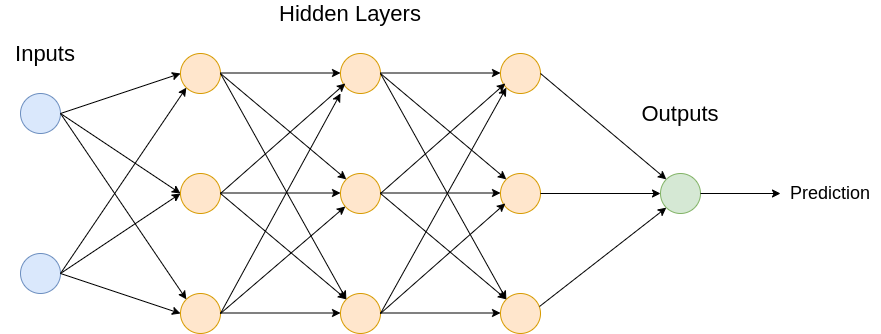
\includegraphics[width=.5\textwidth]{Images/mlp.png}
    \caption{Structure of a Feed-Forward Neural Network.}
    \label{fig:ffnn}
\end{figure}

In a FFNN, perceptrons are organized into 3 types of layers: input, hidden, and
output layers.  Input layers receive the feature vectors as inputs and connect
to the first hidden layer. Hidden layers are intermediate layers that make up
for the bulk of the network. Finally, the output layer is tasked with producing
the result of the network. 

Each layer in a FFNN can have a different number of neurons, and each neuron
within a layer can have a different activation function. It is usual, however,
for neurons in the same layer to have the same activation. 

The number of neurons in the output layer and their activation types depend on
the type of problem being solved. For a regression problem, the network only has
one output neuron, usually with an identity linear activation. In binary
classification problems, one output neuron is sufficient. A sigmoid activation
is also usually used in these cases~\cite{Cybenko1989ApproximationBS}, with
labels 0 and 1 used to represent the two classes. For multi-class
classification, the number of neurons in the output layer matches the number of
classes being identified and a \textit{Softmax}~\cite{pattern_recognition}
(Equation \ref{eq:softmax}) operation is applied to the results of the output
layer neurons' to create a probability distribution vector. The class prediction
is then obtained by obtaining the argmax of such probability vector.

\begin{align}
    \textit{Softmax}(\hat{y}_i) = \frac{e^{\hat{y}_i}}{\sum\limits_j e^{\hat{y}_j}}
    \label{eq:softmax}
\end{align}

Figure~\ref{fig:mlp_solved} shows the decision boundary created by a FFNN with 2
hidden layers of 3 neurons each trained on the dataset discussed previously.

\begin{figure}[!htbp]
    \centering
    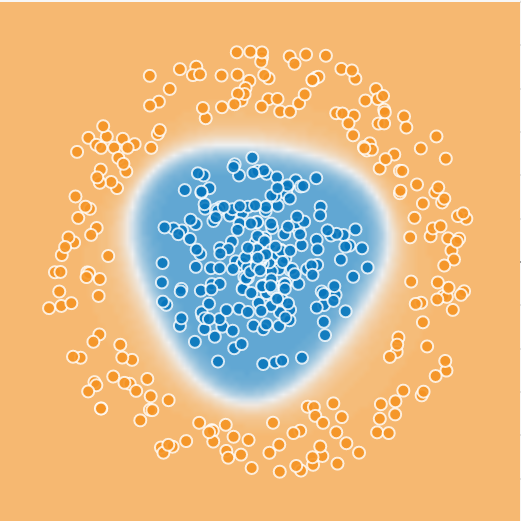
\includegraphics[width=.35\textwidth]{Images/circles_solved.png}
    \caption{Solution with MLP.}
    \label{fig:mlp_solved}
\end{figure}

To make predictions in a FFNN network, the outputs of each layer, also referred
to as \textit{activations}, are obtained sequentially. The activations of the
input layer, obtained using the feature vectors, are in turn used as the inputs
for the first hidden layer. This process known as the \textit{Forward Pass} is
repeated until the activation of the output layer is computed
(Figure~\ref{fig:forward}).

\begin{figure}[!htbp]
    \centering
    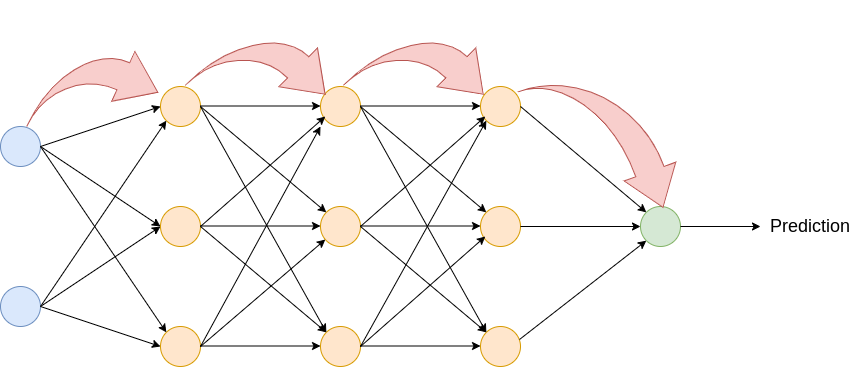
\includegraphics[width=.5\textwidth]{Images/forward_pass.png}
    \caption{Forward pass.}
    \label{fig:forward}
\end{figure}

When using BGD, the forward pass through a FFNN becomes a series of matrix
multiplications. The inputs become a matrix with dimensions $[\textit{Batch\_Size} \times
\textit{\#\_Features}]$ and at each layer, the activations are obtained by multiplying
the input matrix by the weight matrix.
Equations~\ref{eq:forward1}-\ref{eq:forward4} show the forward pass for a
network with 3 hidden layers and one output layer. Note: these equations
purposely omit the neuron's activations as the objective is to highlight the
matrix operations.

\begin{align}
    h_{1_{act}} &= \textit{Inputs} \cdot W_{h_1} \label{eq:forward1}\\
    h_{2_{\textit{act}}} &= h_{1_{\textit{act}}} \cdot W_{h_2} \label{eq:forward2}\\
    h_{3_{\textit{act}}} &= h_{2_{\textit{act}}} \cdot W_{h_3} \label{eq:forward3}\\
    \hat{y} &= h_{3_{\textit{act}}} \cdot W_{O}
    \label{eq:forward4}
\end{align}

Updating the weights in a FFNN is more complex than with a single perceptron.
The loss function merely determines the error at the output layer of the
network. It is then necessary to propagate such error through every layer in the
network all the way back to the input layer. To achieve this, the
\textit{Backpropagation} algorithm~\cite{backprop} is used (Figure~\ref{fig:backprop}).

\begin{figure}[!htbp]
    \centering
    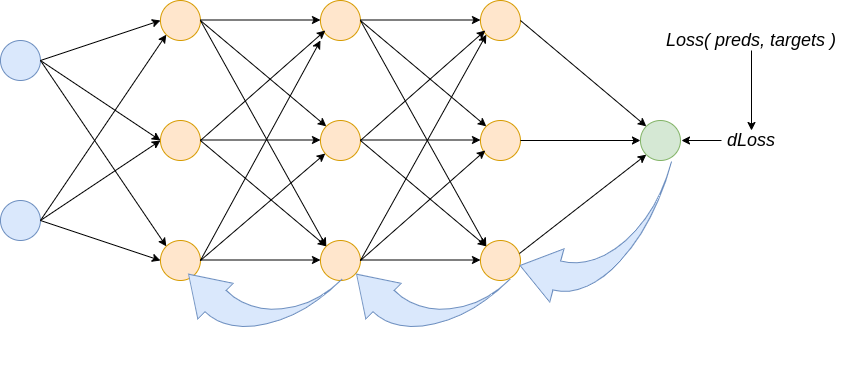
\includegraphics[width=.5\textwidth]{Images/backprop.png}
    \caption{Backpropagation of the error.}
    \label{fig:backprop}
\end{figure}

Once the derivative of the loss function is obtained at the output layer, the
error is propagated back to the preceding layer by multiplying it by the output
layer weights. This same procedure is repeated until the error has reached the
input layer (Equations~\ref{eq:backprop1}-\ref{eq:backprop4}). Note: as before,
these equations omit the derivative of the activation functions as the focus
should be on the matrix operations. 

\begin{align}
    O_{\textit{error}} &= dL_\textit{oss} \label{eq:backprop1}\\
        h_{3_{\textit{error}}} &= O_{\textit{error}} \cdot (W_{O})^T \label{eq:backprop2}\\
        h_{2_{\textit{error}}} &= h_{3_{\textit{error}}} \cdot (W_{h_3})^T \label{eq:backprop3}\\
        h_{1_{\textit{error}}} &= h_{2_{\textit{error}}} \cdot (W_{h_2})^T \label{eq:backprop4}
\end{align}

After the errors for all layers have been computed, the weights can be updated
using the GD formula (Equations~\ref{eq:update1}-\ref{eq:update4}).

\begin{align}
    W_{h_1} &= W_{h_1} - \gamma ((I_\textit{nputs})^T \cdot h_{1_{\textit{error}}}) \label{eq:update1} \\
    W_{h_2} &= W_{h_2} - \gamma ((h_{1_{\textit{act}}})^T \cdot h_{2_{\textit{error}}}) \label{eq:update2} \\
    W_{h_3} &= W_{h_3} - \gamma ((h_{2_{\textit{act}}})^T \cdot h_{3_{\textit{error}}}) \label{eq:update3} \\
    W_{O} &= W_{O} - \gamma ((h_{3_{\textit{act}}})^T \cdot O_{\textit{error}}) \label{eq:update4}
\end{align}

